\documentclass[9pt,dvipdfmx,a4paper]{jsarticle}

\usepackage{amsmath,amssymb}
\usepackage{bm}
\usepackage[dvipdfmx]{graphicx}
\usepackage{physics} % http://mirrors.ibiblio.org/CTAN/macros/latex/contrib/physics/physics.pdf
\usepackage{siunitx} %SI単位を楽に出力
\usepackage{mathtools} %環境の追加
\usepackage{circuitikz} %電気回路をtex中で書く
% \usepackage{caption} %番号なしキャプションを書く
% \usepackage{cancel} %式中に斜線を入れる
% \usepackage{tensor} %テンソルの添え字を書く
% \usepackage{tikz} %図を書く
% \usepackage{ascmac} %四角い枠の中に文章を書く
% \usepackage{float} %figureで[hbp]オプションを使う
% \usepackage{hyperref}  \usepackage{pxjahyper} %ハイパーリンクをつかう
% \usepackage{tablefootnote} %表中に注釈をいれる
% \usepackage[thicklines]{cancel} %数式中の取り消し線
\usepackage[version=4]{mhchem} %化学式の入力
\usepackage{pdfpages}
\usepackage{wrapfig} %文章の回り込み
\usepackage[subrefformat=parens]{subcaption} %(a)図のようにすることができるやつ
\usepackage{here}
\usepackage{mathrsfs} % フォントの追加
\usepackage{url} % url を入れる
\usepackage[margin=15mm]{geometry} %余白の削除
\usepackage{tcolorbox}

\graphicspath{{./image/}}

\begin{document}

%出力したpdfを表紙にするとき
% \includepdf[pages=1,noautoscale=false]{cover.pdf}
% \newpage

%texで表紙を書くとき
\quad\\[35mm]
\centerline{\Huge{\textsf{第 8 回}}}
\quad\\[5mm]
\centerline{\Huge{\textsf{応 用 物 理 学 実 験}}}
\quad\\[5mm]
\begin{table}[h]
	\centering
	\begin{tabular}{| c | c |}
		\hline
		\Huge\textsf{{題目}} & \Huge{\textsf{強誘電体の誘電特性}} \rule[-5mm]{0mm}{15mm} \\
		\hline
	\end{tabular}
\end{table}
\quad\\[10mm]
\begin{table}[h]
	\centering
	\begin{tabular}{l l}
		\hline
		\LARGE{\textsf{氏\qquad 名}} & \LARGE{\textsf{: 西原 翔}} \rule[0mm]{0mm}{6mm} \\
		\hline
		\LARGE{\textsf{学  籍  番  号}} & \LARGE{\textsf{: 1522068}} \rule[0mm]{0mm}{6mm} \\
		\LARGE{\textsf{学部学科学年}} & \LARGE{\textsf{: 理学部第一部応用物理学科3年}}\\
		\hline
	\end{tabular}
\end{table}
\quad\\[10mm]
\centerline{\LARGE{\textsf{共同実験者:1522064 中井空弥}}}\\[2mm]
% \centerline{\LARGE{\textsf{\qquad\qquad\quad\;\;1522091 宮田祟杜}}}\\[2mm]
% \centerline{\LARGE{\textsf{\qquad\qquad\quad\;\;1522095 村山涼矢}}}\\[2mm]
% \centerline{\LARGE{\textsf{\qquad\qquad\quad\;\;1522B02 中村洸太}}}\\[2mm]
\quad\\[10mm]
\centerline{\LARGE{\textsf{提出年月日:2024年11月07日}}}\\[2mm]
\centerline{\LARGE{\textsf{実験実施日:2024年10月25日}}}\\[2mm]
\centerline{\LARGE{\textsf{\qquad\qquad\quad\;2024年11月01日}}}
\quad\\[10mm]
\centerline{\LARGE{\textsf{東 京 理 科 大 学 理 学 部 第 1 部}}}\\[2mm]
\centerline{\LARGE{\textsf{応 用 物 理 学 教 室}}}

\thispagestyle{empty}
\clearpage
\addtocounter{page}{-1}
\newpage

% \twocolumn

\section{Abstract}
本実験ではリン酸二水素カリウム(KDP)について、
試料の温度および入力電場の周波数を変えたときの複素誘電率をLCRメータを用いて測定した。
結果として、110 K から 290 K の範囲における 1 kHz のほとんど直流電場とみなせる入力に対する誘電率の温度依存性、
さらに 130K から 295 K における誘電率の周波数特性を示した。
これらの特性はローレンツモデルをもとにした電場と格子振動が結合したポラリトンによって説明される。
また、Kramers-Kronigの関係式を用いた誘電率の虚部の解析も行い誘電率の虚部を求める方法を比較した。

\section{Introduction}
\subsection*{リン酸二水素カリウム (KDP)}
\begin{wrapfigure}{r}{0.3\columnwidth}
    \centering
    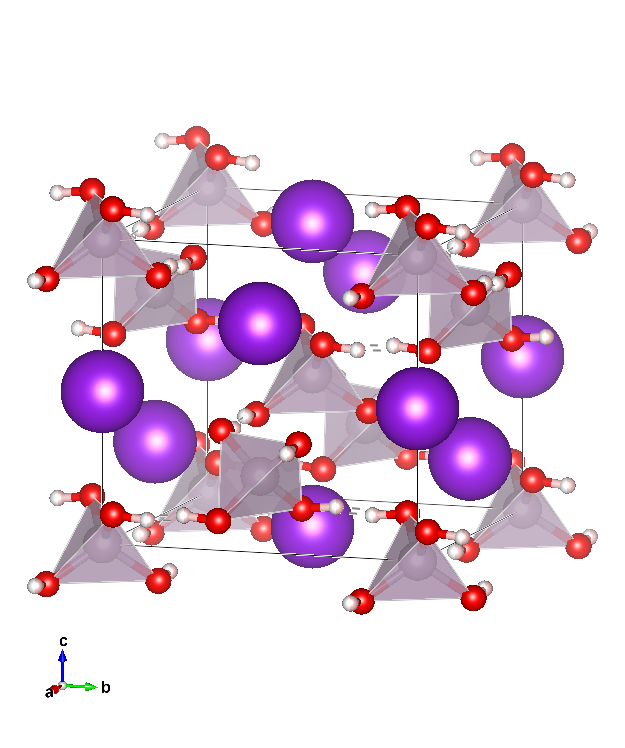
\includegraphics[width = 0.3\columnwidth]{KDP_tetragonal.png}
    \caption{\small{リン酸二水素カリウム(KDP)の結晶構造\cite{cif:7020834}。
    VESTAを用いて作成\cite{VESTA}。}}
    \label{fig:KDP_lattice}
\end{wrapfigure}
強誘電体は電場をかけずとも電気分極持つ材料である。
その分極は外部電場によって反転することができる特徴を持ち、
電場に応じた向きの自発分極を持つようになる。
この特性を活用し、強誘電体はさまざまな応用に利用されている。
光学分野では自発分極による非線形効果を利用して光の振動数や位相、強度を変化させるのに使われる。

今回測定する試料であるリン酸二水素カリウム(KDP)は光学用途に使われる誘電体である。
室温では常誘電体であり強誘電性を用いた光学素子ではないが、
歴史的には初めて発見された強誘電体であるロッシェル塩に次いで発見された強誘電体である。
室温では空間群が \(I-4 2 d\)の正方晶の結晶で、格子定数は a = 4.455, c=6.9266 である(図\ref{fig:KDP_lattice})。
秩序相ではリン酸イオンの配向によって c 軸方向に自発分極を持つことが知られている\cite{onodera}。

この対称性から許される誘電率テンソル
\begin{align}
    \varepsilon_{ij}=\pdv{D_i}{E_j}
\end{align}
の成分を考える。
正方晶の対称操作は a 軸と b 軸の入れ替え、a 軸の反転、 c 軸の反転である。
これらの操作を電束密度\(D\)と電場\(E\)にそれぞれ施すことで
誘電率テンソルが
\begin{align}
    \varepsilon_{ij}=
    \begin{pmatrix}
        \varepsilon_a & 0 & 0\\
        0 & \varepsilon_a & 0\\
        0 & 0 & \varepsilon_c
    \end{pmatrix}
\end{align}
というように書けることがわかる。
今回の実験ではc軸の応答\(\varepsilon_c\)を測定する。


\section{Method}
この実験では KDP の複素誘電率を LCR メータを用いて試料の静電容量\(C_p\)と損失係数\(D\)を測定した。
これと複素誘電率の関係は次のように表せる。
\begin{align}
    \varepsilon_1 - j\varepsilon_2 = \frac{C_p}{C_0}-jD\frac{C_p}{C_0}, \qquad
    C_0 = \frac{\varepsilon_0 S}{d}
\end{align}
ここでの\(S\)は試料の面積、\(d\)は試料の厚さである。
また、LCR メータの測定する仕組みから誘電率の虚部を測定データから実際に求めるのには
\begin{align}
    \varepsilon_2 = D \frac{\abs{C_p}}{C_0}
\end{align}
とする必要がある。これは考察にて言及する。

1 kHz の入力に対する応答の温度変化を 110K から 290 K で測定した。
また、周波数応答を室温では 1kHz から 1MHz まで、
130 K から 295 K では 130 kHz から 190kHz の間で測定した。

また、冷却に関しては液体窒素槽に試料を近づけることで行い、試料の温度は熱電対を用いて測定した。

\clearpage
\section{Result}
1 kHz の入力に対する応答の温度変化を 110K から 290 K で測定した結果が図\ref{graph:epsilon-Temp}のようになった。
112 K において誘電率の実部は最大値をとり、そこからさらに低温では誘電率の値が減っている。
室温における周波数応答は図\ref{graph:epsilon-f_RT}のようになった。

20 kHz で誘電率の変化がみられる。
これは配向分極のモデルであるデバイモデルで説明される変化である。
160 kHz に大きなピークがあり、それより高周波で似た形のピークが確認できる。
これはローレンツモデルによるイオン分極の誘電率の振る舞いである\cite{onodera}。
イオン分極のピークが複数見られるのは、リン酸イオンの振動モードが複数あることに由来すると考えられる。
最も強く応答する周波数こそがその試料の誘電特性を大きく決めるモードであるので、
KDP の誘電率特性を調べる際には 160 kHz 付近を調べればよいのがわかる。
\begin{figure}[t]
    \centering
    \begin{minipage}[t]{0.48\columnwidth}
        \centering
        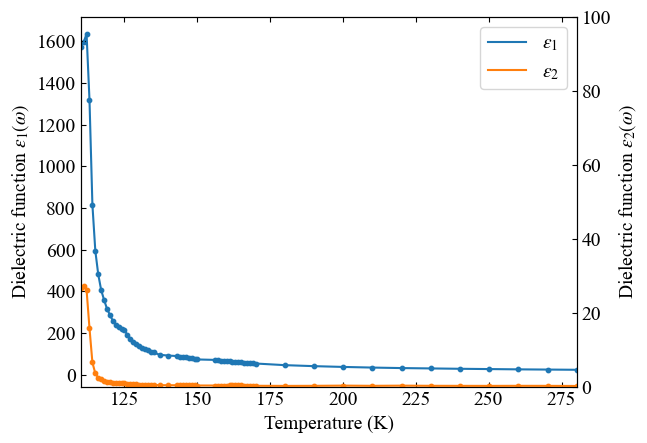
\includegraphics[width = \columnwidth]{epsilon-Temp.png}
        \caption{\small{1 kHz の入力に対する複素誘電率の温度特性。}}
        \label{graph:epsilon-Temp}
    \end{minipage}
    \hfill
    \begin{minipage}[t]{0.48\columnwidth}
        \centering
        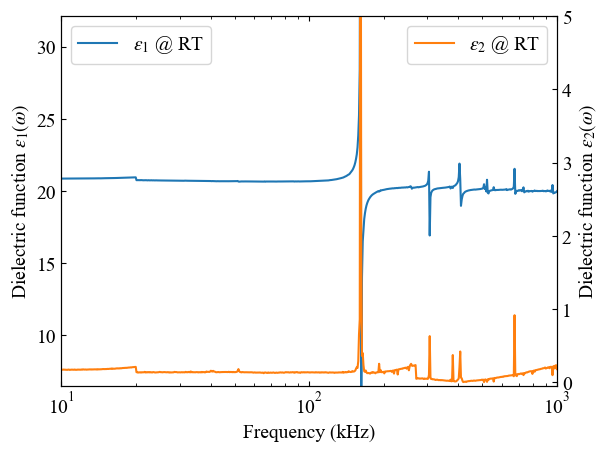
\includegraphics[width = \columnwidth]{epsilon-f_RT.png}
        \caption{\small{室温における複素誘電率の周波数特性。}}
        \label{graph:epsilon-f_RT}
    \end{minipage}\\

    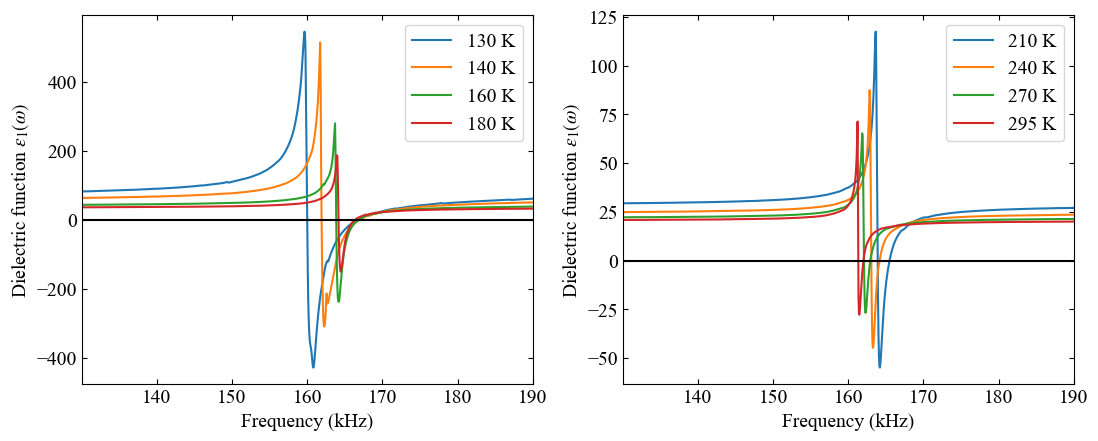
\includegraphics[width=0.96\columnwidth]{epsilon1-f.png}
    \caption{試料の温度を変えたときの誘電率の実部の周波数特性}
    \label{graph:epsilon1-f}
\end{figure}


試料の温度を変えたときの誘電率の実部の周波数特性は図\ref{graph:epsilon1-f}のようになった。
この温度によるピークのの違いはイオン分極の共振周波数が温度によって変わることを表している。
その共振周波数を取り出してプロットしたのが図\ref{graph:ResF-Temp}となる。
180 K で極大値をとり、それより低い温度では下がってるのがわかる。
ただし、イオン分極の性質上、損失係数には必ず2つの大きなピークが生じるため(考察)、
最大のピークではなく、その次に大きいピークを手で選び出す必要がある。

損失係数の周波数特性はを対数プロットすると図\ref{graph:Dissipation-f} のようになった。
様々な周波数でピークが見られる。
160 kHz から 170 kHz にある2つのピーク最も大きく、誘電率の実部が0となるか周波数と対応している。
またそのほかにも小さなペアになったようなピークが認められる。
これは格子振動とのラマン散乱のようなものが見えていると考えられる。

誘電率の虚部を誘電率の実部と損失係数の積から求めると図\ref{graph:epsilon2-f_D},
Kramers-Kronig の関係から求めると図\ref{graph:epsilon2-f_KK}のようになった。
違う方法で求めた両者は値やピークの周波数は同じようになっている。

\begin{figure}[p]
    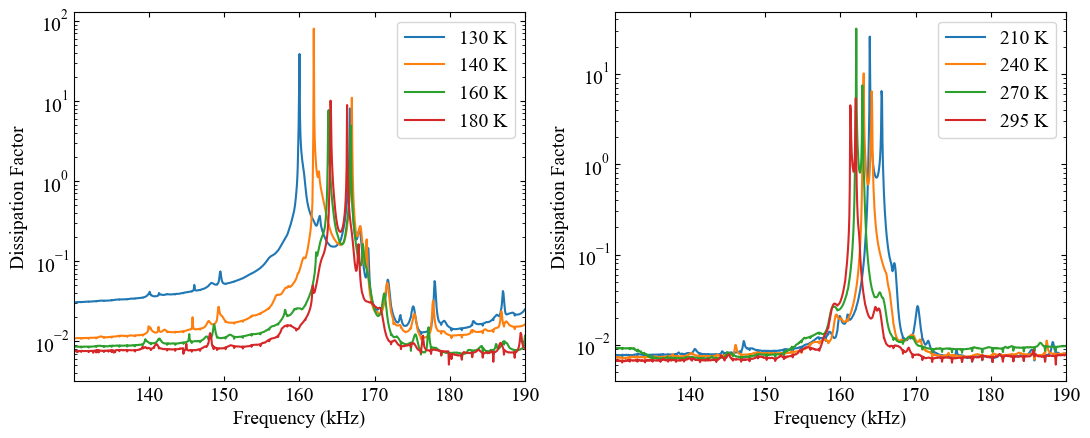
\includegraphics[width=0.96\columnwidth]{Dissipation-f.png}
    \caption{試料の温度を変えたときの損失係数の周波数特性。}
    \label{graph:Dissipation-f}
    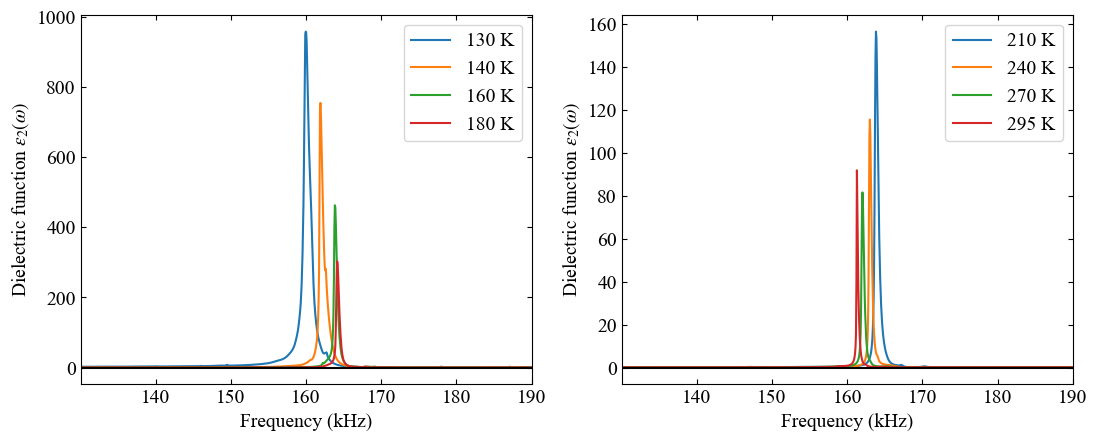
\includegraphics[width=0.96\columnwidth]{epsilon2-f_EpD.png}
    \caption{試料の温度を変えたときの誘電率の虚部の周波数特性。損失係数を使う式(4)を用いた。}
    \label{graph:epsilon2-f_D}
    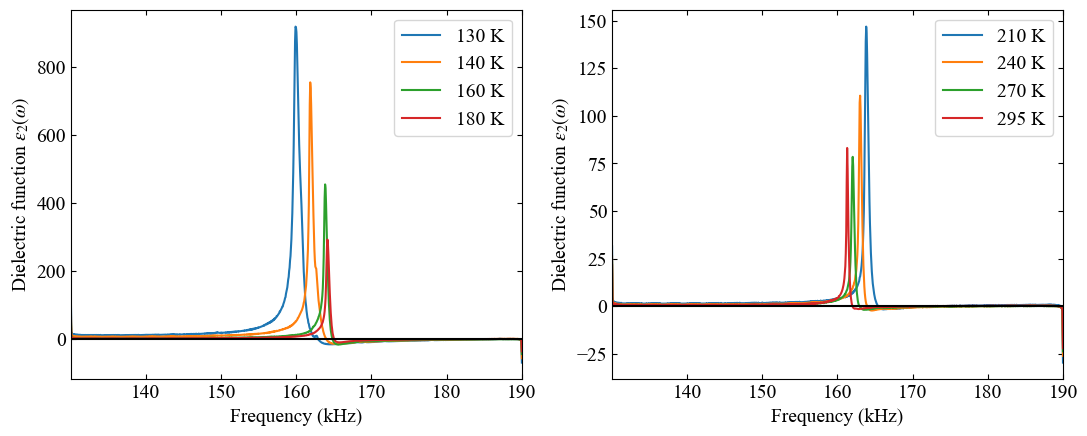
\includegraphics[width=0.96\columnwidth]{epsilon2-f_KK.png}
    \caption{試料の温度を変えたときの誘電率の虚部の周波数特性。
    誘電率の実部を Kramers-Kronig の関係式を使って虚部に変換した。}
    \label{graph:epsilon2-f_KK}
\end{figure}

\section{Discussion}
\subsection{キュリー則}
\begin{figure}[t]
    \centering
    \begin{minipage}[t]{0.48\columnwidth}
        \centering
        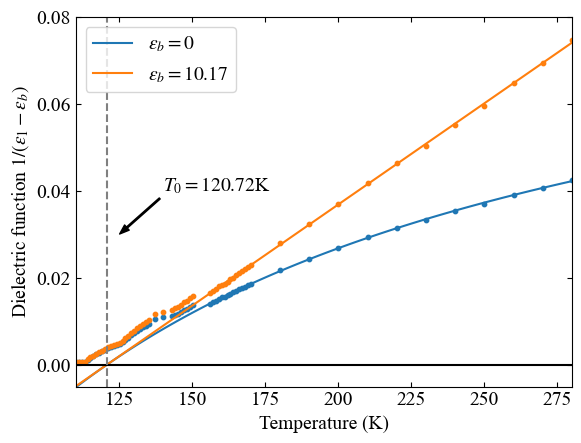
\includegraphics[width = \columnwidth]{1epsilon-Temp.png}
        \caption{\small{1 kHz の入力に対する複素誘電率の実部の逆数の温度特性。
        1kHz は図\ref{graph:epsilon-f_RT}より直流応答とみなすことができる。
        電子分極による背景誘電率\(\varepsilon_b\)を取り除くと直線状になっていることから、
        キュリー則に従っているのがわかる。
        ただし、測定がうまくいかず欠損データや読み取りのずれが大きいところにおける測定データは無視して
        フィッティングを行った。}}
        \label{graph:1epsilon-Temp}
    \end{minipage}
    \hfill
    \begin{minipage}[t]{0.48\columnwidth}
        \centering
        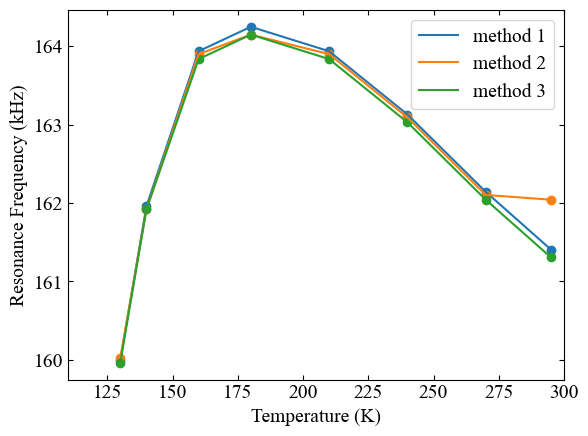
\includegraphics[width = \columnwidth]{ResF-Temp.png}
        \caption{\small{試料の温度を変えたときの、イオン分極の共振周波数様子。
        Method1 は式(4)を用いた複素誘電率の虚部のピークの周波数、
        Method2 は損失係数の最大値を取るときの周波数、
        Method3 は Kramers-Kronig の関係を用いて誘電率の実部から求めた虚部のピークの周波数
        を共振周波数としてプロットした。}}
        \label{graph:ResF-Temp}
    \end{minipage}
\end{figure}

KDP の自発分極はリン酸イオンの双極子モーメントに由来するものである\cite{onodera}。
そのため、秩序・無秩序型の強誘電相転移を起こす物質である。
この相転移はランダウの2次の相転移論を使うことができる。
この系の自由エネルギーは c 軸方向の分極を\(P\)として
\begin{align}
    F = \frac{a(T-T_0)}{2}P^2 + \frac{b}{4}P^4 -pE
\end{align}
と書ける。平衡条件\(\partial F/\partial P = 0\)より
\(E=0\)では
\begin{align}
    P = 0,\quad \pm\sqrt{\frac{a(T_0-T)}{b}}
\end{align}
である。
\begin{align}
    E = a(T-T_0)P + bP^3
\end{align}
両辺を\(P\)で微分することで電気感受率の\(\chi=\partial P/\partial E\)が得られる。
電気感受率と誘電率の関係は\(\varepsilon = \varepsilon_0(1+\chi)\simeq \varepsilon_0\chi\)である。
これより直流電場に対する誘電率は、
\begin{align}
    \varepsilon = \frac{C}{T-T_0}
\end{align}
というような温度特性を示す。
実際の資料では背景に電子分極やほかのイオン分極がある。
これを取り入れると
\begin{align}
    \varepsilon = \varepsilon_b + \frac{C}{T-T_0}
\end{align}
というようになる。これをキュリー則と呼び、定数\(C\)をキュリー定数という。
実際これを確かめるには
\begin{align}
    \frac{1}{\varepsilon-\varepsilon_b} = \frac{T}{C}-\frac{T_0}{C}
\end{align}
というように変形して\(C,\,\varepsilon_b\)実際に直線状になるかを見ればよい。
1kHz は直流とみなせる周波数であるため、
図\ref{graph:epsilon-Temp}でプロットした誘電率の実部を\(\varepsilon\)とみなしてフィッティングをすると
転移温度は\(T_0\) = 120.27 K, 背景誘電率は \(e_b\) = 10.17, キュリー定数は\(C\) = 2152 となった。

\subsection{損失係数から誘電率の虚部を求める式}
複素誘電率の実部と虚部と LCR メータの測定値の関係は
\begin{align*}
    \varepsilon_1 - j\varepsilon_2 = \frac{C_p}{C_0}-jD\frac{\abs{C_p}}{C_0} \tag{(4)'}
\end{align*}
としてあらわされる。
実際この式はうまくいっている。
誘電率の実部は図\ref{graph:epsilon1-f}で見られるようにイオン分極の誘電特性で見られる形をしていて、
誘電率の虚部は図\ref{graph:epsilon2-f_D}は Kramers-Kronig の関係から得られた図\ref{graph:epsilon2-f_KK}
とほとんど同じ値となっている。
しかしよく考えてみると、誘電率の実部が負になるというのは誘電体の静電容量\(C_p\)が負の値を取っているということを表している。
実際そのままの値を使って誘電率の虚部を損失係数との積を取ると
Kramers-Kronig の関係の示すイオン分極の誘電関数の虚部と違った振る舞いを示すため不合理である。
これは何が起きているのか。

これは LCR メータ内の静電容量を測定する仕組みについて考える必要がある。
誘電体にかかっている電場を\(E=E_0\exp(i\omega t)\)としたとき、
内部の電束密度はコンデンサであるため\(D=D_0e^{i(\omega t - \delta)}\)というように位相が遅れる。
Sawyer Tower 法ではこの電束密度は\(D \propto CV\)というように試料の静電容量と電圧という形で
読み取ることができる。いづれにせよ、LCR メータの内部では入力電場と電束密度の位相差を記録することになる。
そうしたときに、この位相差はどのように記録されるかを考える。

素直にどれだけ位相が遅れたかを記録するため\(0\leq \delta \leq 2\pi\)というようにする。
すると2つの信号が同位相であるときには測定誤差により位相の遅れが 0 と \(2\pi\)離れた値を行き来することになる。
それではデータの処理を考える際にはとても扱いにくい値となる。
では\(-\pi\leq\delta\leq\pi\)というように位相差がないときの値の飛びがないように設計すると、
\(\delta>\pi/2\)のときには損失係数を求めるときに不便になる。
損失係数は位相の遅れを\(\tan \delta\)で表すものであり常に正であってほしい量である。
同位相の信号の検出もしながら、損失係数を正に保つには静電容量を負で表すことによって表せばよい。

よって複素誘電率の虚部を求める際には測定された試料の静電容量\(C_p\)の絶対値を取る必要があるのがわかる。

\subsection{共振周波数の求め方}
図\ref{graph:ResF-Temp}で共振周波数を求めてプロットした際、
\begin{enumerate}
    \item 式(4)を使い損失係数を用いて求める方法
    \item 損失係数の最大値をとる方法
    \item Kramers-Kronig の関係をもちいて誘電率の実部から求める方法
\end{enumerate}
の3種類の方法で行った。
いずれの方法でも結果は整合していることからどの方法を使ってもよいことがわかる。
そうなった際、どの解析方法をとればよいかの比較をしてみる。

実験の指導の際に指示されたのは方法1と方法2である。
方法1は LCR メーターの測定データを素直に使った解析方法である。
振動現象を解析する際に基本的に使われる応答の大きさと位相の遅れを見る方法であり、
解析も単に値を掛けるだけで済むため学生実験という目的では適した方法であると思われる。

方法2は損失係数のピークを見るという方法である。
解析は簡単であるが、
Excel を使わず Python 等で自動化すると縦光学フォノンのピークを誤って選び出してしまうことがあるのは注意が必要である。
290 K でのずれはこれによるものである。
さらに、損失係数のピークが何を表しているかは自明ではない。なぜ2つあるピークのうちの左側をとるのか、
ピークの意味は何であるか。これの説明は不十分であり、結果として合うがなぜ合うのかはわからないため、よい解析とは言えない。

方法3は Kramers-Kronig の関係を使った方法である。
複雑な解析ではあるが、この関係式は光学測定によって誘電特性を調べる機器の内部で行われている処理であるため、
一度やってみるというのは面白い方法ではある。
応用物理学科の授業では数値計算が必修となっていないというのもあって、
この実験で数値積分をやるというのも1つの案である。


\subsection{相転移点での誘電率の発散(課題1)}
低温相で自発分極が生じるのは、
周囲からの熱雑音がなく結晶を構成するイオンが特定の向きを向いた基底状態で固定され、
結晶全体で一様な向きに双極子モーメントが揃うことによるものである。
ただし、結晶の単位胞の時点で正味の双極子モーメントが 0 になっていると、
強誘電体とならない。
そして高温になるにつれ自発分極の大きさが小さくなるのは、
振動準位以上の熱雑音によってイオンの向きが乱雑になり、
正味の自発分極が失われていくことによるものである。
これにより転移温度では自発分極の飛びがないような2次相転移となる。

今回の KDP は低温相で直方晶であり、
その内部でのリン酸イオンによる双極子モーメントが c 軸に揃う構造となっているため、
温度を下げると強誘電体となる。
常誘電体で成り立つ関係式
\(P = \varepsilon_0 \chi E\)

が温度を下げ強誘電体になる直前にどのようにどのようになるかを考える。
強誘電体では電場を入力せずとも分極はある。
これを式の上で考えると無限小の入力電場\(E\)を加えたときに有限の分極\(P\)が生じるということになる。
それを満たすためには電気感受率\(\chi\)が発散しなければならない。
\(\chi\)が発散するということは\(\varepsilon = \varepsilon_0(1+\chi)\)であるため誘電率も発散しなければならない。
そのため誘電率は図\ref{graph:epsilon-Temp}のように発散する。

\subsection{損失係数係数の様々なピークと温度特性 (課題2)}
損失係数は誘電率の虚部の情報を持っている。
誘電率の虚部は誘電体の抵抗成分、つまり電流が流れることによる位相変化・エネルギー吸収を表している。
図\ref{graph:Dissipation-f}の 160 kHz から 170 kHz にある2つのピークは誘電率の実部が 0 になる周波数に対応している。
これは格子振動によって説明される。

周波数が低い方のピークはローレンツモデルを拡張したモデルによって説明される。
ローレンツモデルではイオン分極を単一の調和振動子によって説明するものであるが、
実際にはイオンは結晶中であるので単一の調和振動子ではなくバネ格子中にあるとみなすべきである。
バネ格子の頂点にイオンが配置され、そのイオンが外部電場によって強制振動を受ける。
すると外部電場による分極はそのまま格子の変位とみなすことができ、
分極と格子振動が混成する。
これにより、ローレンツモデルでは局所的なバネによる相互作用だけであったが、
格子振動による遠隔相互作用を共振周波数にくりこむことになる。
それは
\begin{align}
    \omega_T^2 = \omega_0^2 - \frac{1}{m}\dfrac{ne^2 /3\varepsilon_0}{1-n\alpha/2}
\end{align}
というようにあらわされる。ここでの\(n\)は電子密度、\(\alpha\)は電子分極である。
これによりローレンツモデルモデルでは説明できなかった共振周波数の温度特性(図\ref{graph:ResF-Temp})
は電子分極の温度特性によるものだと解釈できる。

またもう1つのピークは
誘電率の実部が 0 であるということは\(D = \varepsilon E = \varepsilon_0 E + P\)
より電場を打ち消すような向きに分極が生じている。
電場自体は c 軸方向に周期的に変わっているのでこの分極は c 軸方向に進む縦波になる。
イオン分極による縦波が生成されるということは格子振動となる。
まとめると、損失係数の2つのピークは2種類の光学フォノンの生成を表しているのがわかる。

また余談であるが、試料に格子振動が生じることにより、ラマン散乱で見られるようなストークス線が見えるはずである。
実際、160 kHz から 170 kHz にある2つのピークに対応するようなピークが 145 kHz から 150 kHz と 170 kHz から 180 kHz にある。
つまり、LCR メータの損失係数\(D\)の測定から縦波フォノンのラマン散乱が見えていると考えれる。

\section{Conclusion}
リン酸二水素カリウム (KDP) の試料の温度を変えたときの誘電率が
キュリー則に従うことが確認された。
複素誘電率を測定したところ 160 kHz 付近でイオン分極による共振が確認できた。
また、損失係数のピークは入力電場が縦光学フォノンと横光学フォノンとなって吸収される過程を表している。
これにより、共振周波数の温度特性は横光学フォノンの振動数の表式に含まれる電子分極の温度特性を反映してるのがわかる。
さらに誘電率の虚部を損失係数から求める方法と Kramers-Kronig の関係式を用いた2つの方法で求めたところ一致した。
実験指導では求められないとしていたが、今回の実験の測定データから複素誘電率の虚部を求めることは容易にできることを示した。

\bibliographystyle{junsrt}
\bibliography{reference}
\nocite{*}

\appendix
\section{Kramers-Kronig の関係}
電気感受率の実部と虚部は
\begin{align}
    \chi_2 = -\frac{1}{\pi}\mathcal{P}\int_{-\infty}^{\infty} \frac{\chi_1(\omega')}{\omega'-\omega} d\omega',\qquad
    \chi_1 =  \frac{1}{\pi}\mathcal{P}\int_{-\infty}^{\infty} \frac{\chi_2(\omega')}{\omega'-\omega} d\omega'
\end{align}
という関係がある。
これを Kramers-Kronig の関係式という。
この式はインパルス応答が常に正であるという条件を付けると実部は偶関数、
虚部は奇関数になる。
それを用いると
\begin{align}
    \chi_2 = -\frac{2}{\pi}\mathcal{P}\int_{0}^{\infty} \frac{\omega \chi_1(\omega')}{\omega'^2-\omega^2} d\omega',\qquad
    \chi_1 =  \frac{2}{\pi}\mathcal{P}\int_{0}^{\infty} \frac{\omega'\chi_2(\omega')}{\omega'^2-\omega^2} d\omega'
\end{align}
となる。

Kramers-Kronig の関係式を使って電気感受率の実部の測定データから虚部を求めるには
\begin{align}
    \chi_2
    = -\frac{2}{\pi}\mathcal{P}\int_{0}^{\infty} \frac{\omega \chi_1(\omega')}{\omega'^2-\omega^2} d\omega'\notag
    = -\frac{2f}{\pi}\mathcal{P}\int_{0}^{f_{\mathrm{min}}} \frac{\chi_1(f')}{f'^2-f^2} df'
       -\frac{2f}{\pi}\mathcal{P}\int_{f_\mathrm{min}}^{f_{\mathrm{max}}} \frac{\chi_1(f')}{f'^2-f^2} df'
       -\frac{2f}{\pi}\mathcal{P}\int_{f_\mathrm{min}}^{\infty} \frac{\chi_1(f')}{f'^2-f^2} df'
\end{align}
というように測定データの部分とそれ以外の部分を考えなければならない。
まず測定データに関する積分については
\begin{align}
-\frac{2f_j}{\pi}\mathcal{P}\int_{f_\mathrm{min}}^{f_{\mathrm{max}}} \frac{\chi_1(f')}{f'^2-f_j^2} df'
= -\frac{2f}{\pi}\sum_{i\neq j} \frac{\chi_1(f_i)}{f_i^2-f_j^2}(f_i-f_{i-1})
\end{align}
とすればよい。

それ以外の場所の積分は電気感受率の値は一定であるので
\begin{align}
    -\frac{2}{\pi}\mathcal{P}\int_{0}^{f_{\mathrm{min}}} \frac{f \chi_1(f')}{f'^2-f^2} df'
    = -\frac{\chi_1(f_{\mathrm{min}})}{\pi}\int_{0}^{f_{\mathrm{min}}} \Bigl(\frac{1}{f'-f}-\frac{1}{f'+f}\Bigl) df'
    = -\frac{\chi_1(f_{\mathrm{min}})}{\pi}\ln\Biggl(\frac{f-f_{\mathrm{min}}}{f+f_{\mathrm{min}}} \Biggr)
\end{align}
\begin{align}
    -\frac{2}{\pi}\mathcal{P}\int_{f_{\mathrm{max}}}^{\infty} \frac{f \chi_1(f')}{f'^2-f^2} df'
    = -\frac{\chi_1(f_{\mathrm{min}})}{\pi}\int_{f_{\mathrm{max}}}^{\infty} \Bigl(\frac{1}{f'-f}-\frac{1}{f'+f}\Bigl) df'
    =  \frac{\chi_1(f_{\mathrm{max}})}{\pi}\ln\Biggl(\frac{f_{\mathrm{max}}-f}{f_{\mathrm{max}}+f} \Biggr)
\end{align}
となる。
以上より測定データである誘電率の実部から虚部を求めるには
\begin{align}
    \chi_2(f_j) =
    - \frac{2f}{\pi}\sum_{i\neq j} \frac{\chi_1(f_i)}{f_i^2-f_j^2}(f_i-f_{i-1})
    - \frac{\chi_1(f_{\mathrm{min}})}{\pi}\ln\Biggl(\frac{f-f_{\mathrm{min}}}{f+f_{\mathrm{min}}} \Biggr)
    + \frac{\chi_1(f_{\mathrm{max}})}{\pi}\ln\Biggl(\frac{f_{\mathrm{max}}-f}{f_{\mathrm{max}}+f} \Biggr)
\end{align}
という式を Python や Excel で実装すればよい。

\end{document}